\section{Vulnerarbility Study}
\label{study}
\subsection{Git}
Git's default protocol assumes that all file system operations are ordered. Additionally, Git provides a configuration option (which simply adds \fsyncSC\ calls) that can make Git safer on top of re-ordering file systems. Git's guarantees during a system crash are fuzzy: in catastrophic events, it is assumed that users can do manual recovery by inspecting internal structures in the datastore; however, this is not expected to happen with ordered file systems, or with the fsync-option switched on. We checked Git in the safer mode, with the fsync-option swithced on; note that this reduced performance by about \textbf{150\%} in a simple performance workload.

Our vulnerability-finding workload adds two files to the repository and then commit them. Git's write protocol is modularized (as most applications' are~\cite{tyler}): it has a generic protocol to store an `object', shown in figure~\ref{fig-git-strace}a; the write protocol is then subsequently used while adding and committing. 

 Our checkers invoked read operations on the data store (status, log, show-ref, checkout etc.), write operations (add, rm, commit), and Git's own checker (git-fsck). 

We found vulnerabilities in Git with the fsync-option switched on; some of the vulnerabilities will be exposed on top of widely-used file systems, such as the ext4-ordered mode. Figure~\ref{git-bugs} shows 

\begin{figure*}[t]
\centering
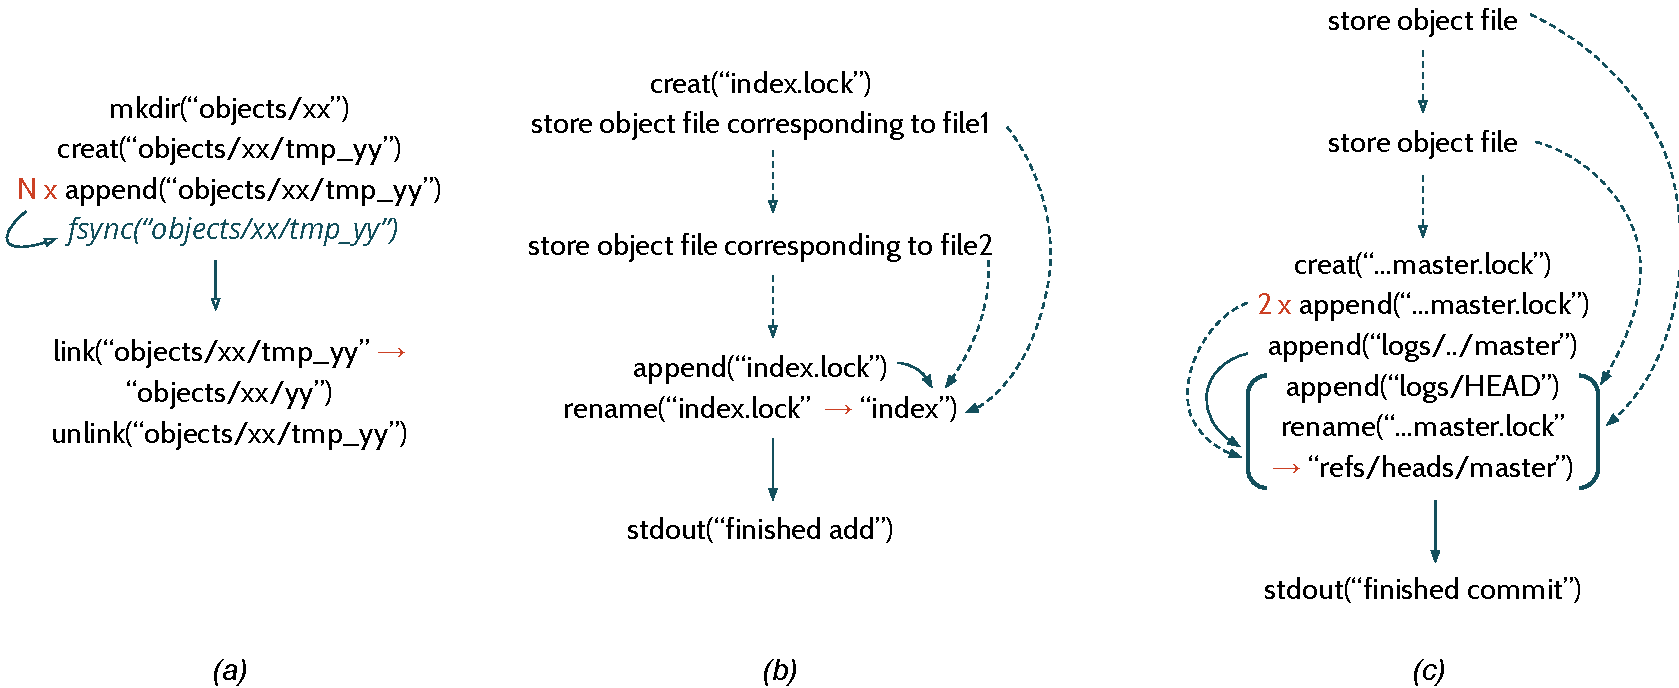
\includegraphics[width=\textwidth]{figs/git_cropped.pdf}
\caption{\textbf{Different parts of the Git protocol. }\textit{\footnotesize (a) shows how Git creates and stores an `object' in its data store. (b) and (c) show the full add and commit protocols, respectively. The fsync() in (a) happens only if Git is configured to expect an unordered file system. The arrows with a hollow arrow-point show user-specified orderings because of fsync(), and arrows with solid arrow-points show required orderings. Arrows that drop down straight are because of fsync(): they convey that the fsync() is ordered before all subsequent calls; curved arrows show fine-grained orderings, of only particular calls being ordered. Dotted arrows show when only part of a group of system calls are concerned with ordering. For example, the topmost, straight-down dotted arrow in (b) shows that only parts of the object file creation are ordered by the fsync(): the link() and mkdir() are not ordered. The topmost curved arrow in (b) shows that only parts of the object file creation \emph{need} to be ordered before the rename(): the creat() in (a) need not be ordered, while the link() should be. The brackets in (c) show required atomicity.}}
\label{fig-git-strace}
\end{figure*}

